\chapter{Planning}

Planning the works needs no introduction, but the reality is that most Engineers
do very little planning of their works whereas many others understand that planning
is something done at the beginning of a Project using Primavera and the rest is just following the direction of the Project as it goes.

There are many elements of planning and before we get onto that we will analyse them in details. In many respects planning is like waterpainting, you start sketiching to see what you want to achieve and then you detail it as you go along.

\begin{fullwidth}
\begin{figure*}
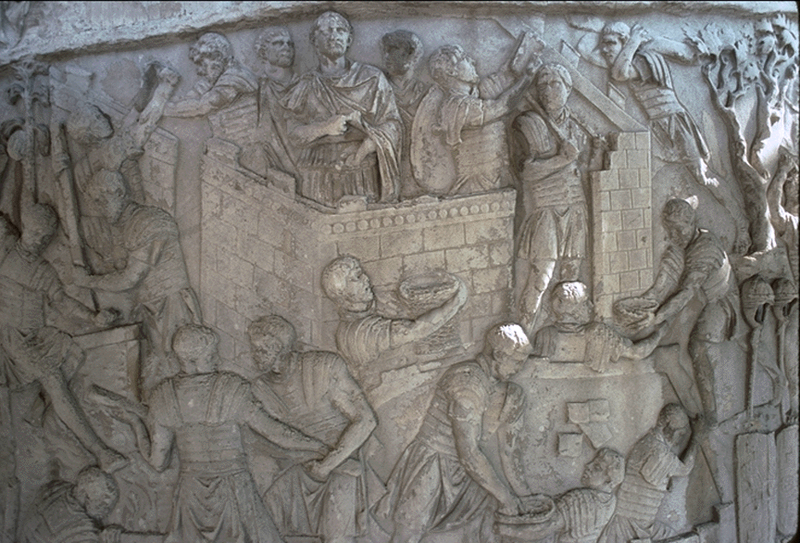
\includegraphics[width=1.1\textwidth]{./graphics/trajan-column}
\caption{Roman soldiers building a fortress, Trajan's Column 113 AD}
\end{figure*}
\end{fullwidth}

Planning is both the organizational process of creating and maintaining a \textit{plan}; and the psychological process of thinking about the activities required to create a desired goal.

\section*{Determining the right sequence of works}

Before any plan is drawn some understanding of the sequence of works
is necessary. Activities can be divided into sequential or parallel. A
sequential activity is one that you cannot start unless a previous activity
has been completed. If the activity of having procured the materials is not
completed, then the works cannot be started. 

\section*{How do I start}

The first thing you need to do before you start is to identify the \textit{goal}.
In many cases this is not that difficult, but you will find out that the goal as
stated is too theoretical and you need to cut it down to smaller objectives.

We will discuss techniques by means of focusing on examples which are smaller.
In my opinion this is where most people fail to plan properly and let events
overtake them. We will assume that shop drawings are available and that materials
are also available and that we will use a Team of Duct erectors.

\subsection*{Measure your target}

Unless you measure something, you cannot control it. If you know that you have to install 600 m$^2$ of ductwork, you may be in a better position to estimate the time
it takes to install it (provided that you have some background information). 


\begin{marginfigure}
The Tower can be represented by a series of squares, which denote an activity. Green is done and white is not done. There is no need to use intermediate colors. they just detract from the visual information.
\vspace{1cm}
%% Color definitions




\floor{Level 47}{0}{0}{0}{0}{2}
\floor{Level 46}{0}{0}{0}{2}{2}
\floor{Level 45}{0}{0}{1}{1}{1}
\floor{Level 44}{0}{0}{1}{1}{1}
\floor{Level 43}{1}{1}{1}{1}{1}
\floor{Level 42}{1}{1}{1}{1}{1}
\floor{Level 41}{0}{1}{1}{0}{1}
\floor{Level 40}{0}{1}{1}{1}{1}
\floor{Level 39}{0}{1}{1}{1}{1}
\floor{Level 38}{0}{1}{1}{1}{1}
\floor{Level 37}{0}{0}{1}{1}{1}
\floor{Level 36}{0}{0}{0}{1}{1}
\floor{Level 35}{0}{0}{0}{1}{1}
\floor{Level 34}{0}{0}{0}{1}{1}
\floor{Level 33}{0}{0}{0}{1}{1}
\floor{Level 32}{0}{0}{0}{1}{1}
\floor{Level 31}{0}{0}{0}{1}{1}
\floor{Level 30}{0}{0}{0}{1}{1}
\floor{Level 29}{1}{1}{1}{1}{1}
\floor{Level 28}{1}{1}{1}{1}{1}
\floor{Level 27}{0}{1}{1}{1}{1}
\floor{Level 26}{0}{1}{1}{1}{1}
\floor{Level 25}{0}{0}{1}{1}{1}
\floor{Level 24}{0}{0}{1}{1}{1}
\floor{Level 23}{0}{0}{1}{1}{1}
\floor{Level 22}{0}{0}{1}{1}{1}
\floor{Level 21}{0}{0}{1}{1}{1}
\floor{Level 20}{0}{0}{1}{1}{1}
\floor{Level 19}{0}{0}{1}{1}{1}
\floor{Level 18}{0}{0}{1}{1}{1}
\floor{Level 17}{0}{0}{1}{1}{1}
\floor{Level 16}{0}{0}{1}{1}{1}
\floor{Level 15}{0}{1}{1}{1}{1}
\floor{Level 14}{0}{1}{1}{1}{1}
\floor{Level 12}{0}{1}{1}{1}{1}
\floor{Level 11}{0}{1}{1}{1}{1}
\floor{Level 10}{1}{1}{1}{1}{1}
\floor{Level 09}{1}{1}{1}{1}{1}
\floor{Level 08}{1}{1}{1}{1}{1}




%
%\begin{tikzpicture}[scale=0.8]
%\draw node [anchor=south east]{Level 08};
%\draw (0,0) rectangle (0.5,0.5);
%\draw  [fill=green] (0.6,0.0) rectangle (1.1,0.5) ;
%\draw [fill=green] (0.6+0.6,0.0) rectangle (1.7,0.5) ;
%\draw[fill=green]  (3*0.6,0.0) rectangle (2.3,0.5) ;
%\draw[fill=green]  (4*0.6,0.0) rectangle (2.9,0.5) ;
%\node at (4,0.1) {Apart. 90\%};
%\end{tikzpicture}
%\def\addlegend#1#2{% color label
%  \begin{tikzpicture}[scale=0.8]
%   \draw[fill=#1] (0,0) rectangle (0.5,0.5);
%   \draw node [anchor=south east]{#2};
%   \end{tikzpicture}\vspace{2pt}}
%\addlegend{green}{lights}
\caption{Rotana Tower Progress, each square represents one separate activity}
\end{marginfigure}


When you first start with the plan, a visual representation of the
areas and work you will be working on can be invaluable. For example
a layout of the area with some coloring can help you identify better
to visualize the problem. At this point if the area is available, you
should visit the area and get a feeling of the problems that you may 
encounter. Once you have a good idea of what you want to achieve, you need to translate
it into something more definable. For ductwork we would normally divide
the work as shown in \ref{ductplan}. For most MEP activities is almost
a rule that unless you put a Team to start by installing supports, it is 
almost certain that manhours will be lost later on. By starting supports early
you ensure that the charge-hand who is marking the support locations is
scouting the area and ensuring that there are no impediments. In very rare
occassions that this is not necessary, such as ductwork in plantrooms.

\pagebreak
\gdef\ascale{0.65}
\begin{minipage}{4cm}
\small
\floor{Level 47}{0}{0}{0}{0}{2}
\floor{Level 46}{0}{0}{0}{2}{2}
\floor{Level 45}{0}{0}{1}{1}{1}
\floor{Level 44}{0}{0}{1}{1}{1}
\floor{Level 43}{1}{1}{1}{1}{1}
\floor{Level 42}{1}{1}{1}{1}{1}
\floor{Level 41}{0}{1}{1}{0}{1}
\floor{Level 40}{0}{1}{1}{1}{1}
\floor{Level 39}{0}{1}{1}{1}{1}
\floor{Level 38}{0}{1}{1}{1}{1}
\floor{Level 37}{0}{0}{1}{1}{1}
\floor{Level 36}{0}{0}{0}{1}{1}
\floor{Level 35}{0}{0}{0}{1}{1}
\floor{Level 34}{0}{0}{0}{1}{1}
\floor{Level 33}{0}{0}{0}{1}{1}
\floor{Level 32}{0}{0}{0}{1}{1}
\floor{Level 31}{0}{0}{0}{1}{1}
\floor{Level 30}{0}{0}{0}{1}{1}
\floor{Level 29}{1}{1}{1}{1}{1}
\floor{Level 28}{1}{1}{1}{1}{1}
\floor{Level 27}{0}{1}{1}{1}{1}
\floor{Level 26}{0}{1}{1}{1}{1}
\floor{Level 25}{0}{0}{1}{1}{1}
\floor{Level 24}{0}{0}{1}{1}{1}
\floor{Level 23}{0}{0}{1}{1}{1}
\floor{Level 22}{0}{0}{1}{1}{1}
\floor{Level 21}{0}{0}{1}{1}{1}
\floor{Level 20}{0}{0}{1}{1}{1}
\floor{Level 19}{0}{0}{1}{1}{1}
\floor{Level 18}{0}{0}{1}{1}{1}
\floor{Level 17}{0}{0}{1}{1}{1}
\floor{Level 16}{0}{0}{1}{1}{1}
\floor{Level 15}{0}{1}{1}{1}{1}
\floor{Level 14}{0}{1}{1}{1}{1}
\floor{Level 12}{0}{1}{1}{1}{1}
\floor{Level 11}{0}{1}{1}{1}{1}
\floor{Level 10}{1}{1}{1}{1}{1}
\floor{Level 09}{1}{1}{1}{1}{1}
\floor{Level 08}{1}{1}{1}{1}{1}
\end{minipage}
\hspace{1em}
\begin{minipage}{4cm}
\small
\floor{Level 47}{0}{0}{0}{0}{2}
\floor{Level 46}{0}{0}{0}{2}{2}
\floor{Level 45}{0}{0}{1}{1}{1}
\floor{Level 44}{0}{0}{1}{1}{1}
\floor{Level 43}{1}{1}{1}{1}{1}
\floor{Level 42}{1}{1}{1}{1}{1}
\floor{Level 41}{0}{1}{1}{0}{1}
\floor{Level 40}{0}{1}{1}{1}{1}
\floor{Level 39}{0}{1}{1}{1}{1}
\floor{Level 38}{0}{1}{1}{1}{1}
\floor{Level 37}{0}{0}{1}{1}{1}
\floor{Level 36}{0}{0}{0}{1}{1}
\floor{Level 35}{0}{0}{0}{1}{1}
\floor{Level 34}{0}{0}{0}{1}{1}
\floor{Level 33}{0}{0}{0}{1}{1}
\floor{Level 32}{0}{0}{0}{1}{1}
\floor{Level 31}{0}{0}{0}{1}{1}
\floor{Level 30}{0}{0}{0}{1}{1}
\floor{Level 29}{1}{1}{1}{1}{1}
\floor{Level 28}{1}{1}{1}{1}{1}
\floor{Level 27}{0}{1}{1}{1}{1}
\floor{Level 26}{0}{1}{1}{1}{1}
\floor{Level 25}{0}{0}{1}{1}{1}
\floor{Level 24}{0}{0}{1}{1}{1}
\floor{Level 23}{0}{0}{1}{1}{1}
\floor{Level 22}{0}{0}{1}{1}{1}
\floor{Level 21}{0}{0}{1}{1}{1}
\floor{Level 20}{0}{0}{1}{1}{1}
\floor{Level 19}{0}{0}{1}{1}{1}
\floor{Level 18}{0}{0}{1}{1}{1}
\floor{Level 17}{0}{0}{1}{1}{1}
\floor{Level 16}{0}{0}{1}{1}{1}
\floor{Level 15}{0}{1}{1}{1}{1}
\floor{Level 14}{0}{1}{1}{1}{1}
\floor{Level 12}{0}{1}{1}{1}{1}
\floor{Level 11}{0}{1}{1}{1}{1}
\floor{Level 10}{1}{1}{1}{1}{1}
\floor{Level 09}{1}{1}{1}{1}{1}
\floor{Level 08}{1}{1}{1}{1}{1}
\end{minipage}
\hspace{0.8cm}
\begin{minipage}{4cm}
\small
\floor{Level 47}{0}{0}{0}{0}{2}
\floor{Level 46}{0}{0}{0}{2}{2}
\floor{Level 45}{0}{0}{1}{1}{1}
\floor{Level 44}{0}{0}{1}{1}{1}
\floor{Level 43}{1}{1}{1}{1}{1}
\floor{Level 42}{1}{1}{1}{1}{1}
\floor{Level 41}{0}{1}{1}{0}{1}
\floor{Level 40}{0}{1}{1}{1}{1}
\floor{Level 39}{0}{1}{1}{1}{1}
\floor{Level 38}{0}{1}{1}{1}{1}
\floor{Level 37}{0}{0}{1}{1}{1}
\floor{Level 36}{0}{0}{0}{1}{1}
\floor{Level 35}{0}{0}{0}{1}{1}
\floor{Level 34}{0}{0}{0}{1}{1}
\floor{Level 33}{0}{0}{0}{1}{1}
\floor{Level 32}{0}{0}{0}{1}{1}
\floor{Level 31}{0}{0}{0}{1}{1}
\floor{Level 30}{0}{0}{0}{1}{1}
\floor{Level 29}{1}{1}{1}{1}{1}
\floor{Level 28}{1}{1}{1}{1}{1}
\floor{Level 27}{0}{1}{1}{1}{1}
\floor{Level 26}{0}{1}{1}{1}{1}
\floor{Level 25}{0}{0}{1}{1}{1}
\floor{Level 24}{0}{0}{1}{1}{1}
\floor{Level 23}{0}{0}{1}{1}{1}
\floor{Level 22}{0}{0}{1}{1}{1}
\floor{Level 21}{0}{0}{1}{1}{1}
\floor{Level 20}{0}{0}{1}{1}{1}
\floor{Level 19}{0}{0}{1}{1}{1}
\floor{Level 18}{0}{0}{1}{1}{1}
\floor{Level 17}{0}{0}{1}{1}{1}
\floor{Level 16}{0}{0}{1}{1}{1}
\floor{Level 15}{0}{1}{1}{1}{1}
\floor{Level 14}{0}{1}{1}{1}{1}
\floor{Level 12}{0}{1}{1}{1}{1}
\floor{Level 11}{0}{1}{1}{1}{1}
\floor{Level 10}{1}{1}{1}{1}{1}
\floor{Level 09}{1}{1}{1}{1}{1}
\floor{Level 08}{1}{1}{1}{1}{1}
\end{minipage}

\pagebreak
\def\don#1{\cellcolor[gray]{0.9}#1}  %{0.9}
\setcounter{inc}{0} % reset counter
\begin{table}[htbp]
\vspace{0.8cm}
\small
\begin{tabular}{|l|p{3.9cm}|l|l|l|l|l|l|l|l|}
\hline
item  &Description  &Qty   &Week 1 &Week 2 &Week 3 &Week 4 &Week 5 &Week 6 &Total\\
\hline
\inc     &supports &400 &\don{100} &\don{100} &\don{100} &\don{100} & & &\\
\inc     &ductwork (insulated) &1200 &\don{200} &\don{200} &\don{200} &\don{200} &\don{200} &\don{200} &\\
\inc     &ductwork (uninsulated) & 600 & & & & & & &\\
\inc     &vol. dampers & & & & & & & &\\
\inc     &fire dampers & & & & & & & &\\
\inc     &flexibles & & & & & & & &\\
\inc     &WIR   & & & & & & & &\\      
\hline
\end{tabular}
\caption{Example of 6 week look-ahead program for installation of ductwork.}
\label{ductplan}
\end{table}

\setcounter{inc}{0} % reset counter
\begin{table}[htbp]
\vspace{0.8cm}
\small
\begin{tabular}{|l|p{3.9cm}|l|l|l|l|l|l|l|l|}
\hline
item  &Description  &qty   &unit & manhours &$f_1$ &$f_2$ &$f_3$ &$f_4$ &Total\\
\hline
\inc     &supports &400 &each & & & & & &\\
\inc     &ductwork (insulated) &1200 &m$^2$ & & & & & &\\
\inc     &ductwork (uninsulated) & 600 &m$^2$ & & & & & &\\
\inc     &vol. dampers &80 &each & & & & & &\\
\inc     &fire dampers &20 &each & & & & & &\\
\inc     &flexibles &60 &each & & & & & &\\
\inc     &WIR   &5 &each & & & & & &\\      
\hline
\end{tabular}
\caption{Example of 6 week look-ahead program for installation of ductwork.}
\label{ductplan}
\end{table}


The factors $f_1, f_2, f_3, f_4$ are a series of factors that ca be used to
adjust your estimate based on your observations of the rate of the works and
the actual conditions that the work is taking place.

$f_1$ = congestion factor.

$f_2$ = weather factor.

$f_3$ = team expertise.

$f_4$ = overtime work.

Of importance is to note that your budget for overtime works will increase
the total manhours that are required to complete the works, as overtime work
in general reduces efficiency of personnel.

The above costs are estimated to be on the low side. Published tables are frequently used to quantify loss of productivity for scheduled overtime [18,19,20,21], overmanning [22,23,24], congestion of trades [23], remobilization [22], and weather [25,26,27].

In this Project the Contractor accelerated completion activities in many areas in order to follow the program. Loss of productivity occurred as a result of overtime due to a number of reasons: fatigue; demotivation; absenteeism; reduction of workpace and congestion, see Figure \ref{fig:congestion}; The factors most commonly cited in the literature are those prepared by the Construction Users' Anti-Inflation Roundatable\sidenote{Construction Users' Anti-Inflation Roundtable, `'Overtime in Construction'', AACE Bulletin, Vol. 15, No. 5, October 1973.}, shown in Figure \ref{fig:overtime}. These impacts have not be taken into account in the above calculations, as the Contractor was aware that overtime, however, inefficient had to be introduced to complete the works by the agreed date. However, not all these costs belong to the Contractor as the Contractor attempted to coomplete Engineer's Instructions and other changes as quick as possible.


\begin{figure}[htbp]
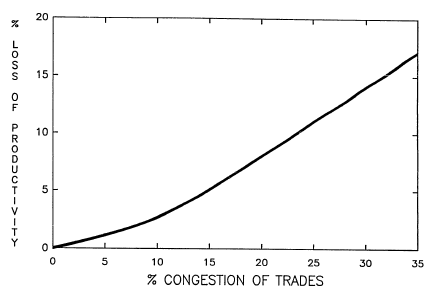
\includegraphics[width=0.9\textwidth]{./graphics/AHU/congestion}
\caption{Impact of overtime on productivity}
\label{fig:overtime}
\end{figure}


\begin{figure}[htbp]
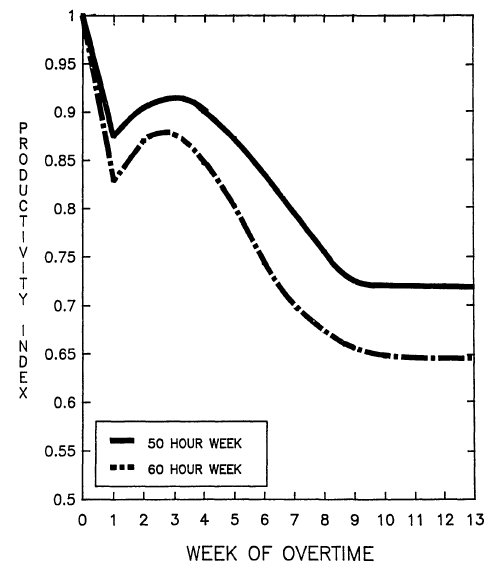
\includegraphics[width=0.8\textwidth]{./graphics/AHU/overtime}
\caption{Impact of overtime on productivity}
\label{fig:congestion}
\end{figure}


The major cause of schedule disruptions and delays all related to lack of information and change orders. Essentially, all causes beyond the Contractor's control

\subsection{Resourcing}

The first step that we discussed so far is how to analyze an activity and
produce a rough estimate of the man-hours required to complete the works.
In the second Table we have added some factors that can assist to determine
productivity; when they are applied they will either increase or decrease
the estimate. 

Once this step has been completed, we need to allocate the necessary resources
to the activity, that is alloacte technicians that are going to carry out the
installation.

My suggestion: when you need to structure a big project, don’t impose a \textit{preferred team} size on people just because it is written in a book. Try to allow self-organization to do its job and let the people (within their real environment) figure out what their optimum is. Do they want to cut a team of seven into two teams of three and four? Sure, why not? Are they merging two teams into one big team of fifteen? Fine, let them see if that works. And be aware that they might want to reconsider things when the environment (or the set of personalities in the team) changes again.

In general though use what it works, but allocate the teams.

A charge-hand can handle up to a 'tent-group' well which should be 5-9 people. We will call these groups, by letters

Ducting Group A

Ducting Group B

Ducting Group C

Ducting Group D

Ducting Group E


\subsection*{The ideal size of a group}

The two-pizza principle can be used to determine an ideal group size. Simply
stated is that you should be able to feed this group with two-pizzas. \sidenote{
Jeff Bezos, has been quoted at \url{http://www.fastcompany.com/magazine/85/bezos_4.html}.} For ductwork
the suggestion is to use 12 people per charge-hand. The rationale behind this
is that this is the maximum size group that a charge-hand can handle well. It
divides into 3 smaller groups of four, which makes installation of heavier
ductwork easier. During third fix activities, it can be split into six pairs
for installation of diffusers.

Some rule of thumbs to allow for ductwork installation that is fully inclusive
of all grilles, diffusers and the like is that you can get a productivity of
approximately 1 m$^2$ per worker. So if you had a full Team able to install 
ductwork for 12 months, out of a 24 month Project to install 100,000 m$^2$ of
ductwork you will need.

\[ n = \frac{100000}{260 \times 12 \times f_1 \times f_2 \times f_3}   \]


If the productivity factors were set to 1 it would require 32 men. Of course the
above is ideal, where one assumes that the workers are working the full day
in ductwork installation, there are are no delays that reduce the productivity.
However, keep this in mind. The other issue is factors relating to the learning
curve and also the fact that work does not always lend it self to a constant
production rate. For smaller ductwork productivity really drops to about less
than half of the above ideal. This also excludes manufacturing of special pieces
tha that necessary, connection of equipment and the like. Those should rather
be measured as individual pieces.

\subsection*{Subdividing the work}

We briefly touched, while discussing productivity factors on the subject
of the \textit{learning curve}. The concept of the learning curve was introduced to the aircraft industry in 1936 when T. P. Wright published an article in the February 1936 Journal of the Aeronautical Science. Wright described a basic theory for obtaining cost estimates based on repetitive production of airplane assemblies. Since then, learning curves (also known as progress functions) have been applied to all types of work from simple tasks to complex jobs like manufacturing a Space Shuttle.

The theory of learning is simple. It is recognized that repetition of the same operation results in less time or effort expended on that operation. For the Wright learning curve, the underlying hypothesis is that the direct labor man-hours necessary to complete a unit of production will decrease by a constant percentage each time the production quantity is doubled. If the rate of improvement is 20\% between doubled quantities, then the learning percent would be 80\% (100-20=80). While the learning curve emphasizes time, it can be easily extended to cost as well.

This simple and now widely accepted principle should be leveraged in your
production planning. For example on high-rise buildings, one should plan
the work vertically, for example one group doing the same activity as they
are going up the Tower See the \ref{towerplan}.

Although, technicians are trained in what they do, the fact that just by moving
around in different areas of the building in unfamiliar surroundings keeps
on affecting productivity. So the rule is to try and plan the works in such
a way that you get the benefit of productivity improvements by using 
repetitive tasks.

\section*{The Gant Chart}

So far we have discussed a number of visual tools and tabular methods to help
assess and plan the works. These are important tools for day to day work and
for work spanning up to six weeks of planning. However, tempting to extend them
to longer periods these will tend to fail as the amount of complexity you adding
prohibits people from understanding them well. In addition if the plan needs
revisions they take took long to modify that one will lose any benefit from
such updates.



%%
% MERWEB TOWER PROGRESS REPORT

\small
\begin{table}[p]
\caption{Merweb Ceiling and Wall Closure Plan}
\begin{tabular}{llllll}
\toprule 
\multicolumn{6}{c}{\bf Merweb Ceiling and Wall Closure}\\
\midrule
~        & Corridor & Pass. lift  & Serv. lift  & Rooms   & Dry walls \\
Level   &            & lobby             &lobby    &    &              \\ 
\midrule
Lvl 43  &             &                &                &             &              \\
Lvl 41  &             &              &         &     &        \\
Lvl 40  & \done     &\done&\done&\done&\done\\
Lvl 39  & \done     &\done&\done&\done&\done\\
Lvl 38  & \done     &\done&\done&\done&\done\\
Lvl 37  & \done     &\done&\done&\done&\done\\
Lvl 36  & \done     &\done&\done&\done&\done\\
Lvl 35  & \done     &\done&\done&\done&\done\\
Lvl 34  & \done     &\done&\done&\done&\done\\
Lvl 33  & \done     &\done&\done&\done&\done\\
Lvl 32  & \done     &\done&\done&\done&\done\\
Lvl 31  & \done     &\done&\done&\done&\done\\
Lvl 30  & \done     &\done&\done&\done&\done\\
Lvl 29  & \done     &\done&\done&\done&\done\\
Lvl 28  & \done     & 27 Jul          &27 Jul         &27 Jul        &\done\\
Lvl 27  & 29 Jul    & 29 Jul   &29 Jul         &29 Jul         &\done \\
Lvl 26  & 2 Aug    & 2 Aug  & 2 Aug        &2 Aug         &\done \\
Lvl 25  & 4 Aug    & 4 Aug  & 4 Aug        &4 Aug         &\done \\
Lvl 24  & 7 Aug    & 7 Aug  & 7 Aug        &7 Aug         &\done \\
Lvl 23  & 9 Aug    & 9 Aug  & 9 Aug        &9 Aug         & 24 Jul\\
Lvl 22  & 11 Aug   &11 Aug & 11 Aug        &11 Aug         &26 Jul\\
Lvl 21  & 14 Aug   &14 Aug  & 14 Aug        &14 Aug         &28 Jul\\
Lvl 20  & 16 Aug   &16 Aug          &16 Aug         &16 Aug         &30 Jul\\
Lvl 19  & 18 Aug   &18 Aug           &18 Aug         &18 Aug         &1 Aug\\
Lvl 18  & 21 Aug   &21 Aug & 21 Aug                  &21 Aug         &3 Aug\\
Lvl 17  & 23 Aug   &23 Aug  &23 Aug         &23 Aug         &5 Aug\\
Lvl 16  & 25 Aug   &25 Aug  &25 Aug         &25 Aug         &7 Aug\\
Lvl 15  & 27 Aug   &27 Aug  &27 Aug         &27 Aug         &9 Aug\\
Lvl 14  & 30 Aug   &30 Aug  &30 Aug         &30 Aug         &11 Aug\\
Lvl 13  & 1 Sep     &1 Sep  &1 Sep         &1 Sep         &13 Aug\\
Lvl 12  & 4 Sep     &4 Sep  & 4 Sep        &4 Sep         &15 Aug\\
Lvl 11  & 6 Sep     &6 Sep  & 6 Sep        &6 Sep         &17 Aug\\
Lvl 10  & 8 Sep     &8 Sep  & 8 Sep        &8 Sep         &19 Aug\\
Lvl 09  & 10 Sep   &10 Sep  & 11 Sep        &11 Sep         &21 Aug\\
Lvl 08  & 12 Sep   &12 Sep  & 13 Sep        &13 Sep         &23 Aug\\
Lvl 07  & 15 Sep   &15 Sep  & 15 Sep        &15 Sep         &25 Aug\\
\bottomrule
\end{tabular}
\normalsize
\label{towerplan}
\end{table}
\normalsize

A Gantt chart is a type of bar chart that illustrates a project schedule. Gantt charts illustrate the start and finish dates of the terminal elements and summary elements of a project. Terminal elements and summary elements comprise the work breakdown structure of the project. Some Gantt charts also show the dependency (i.e., precedence network) relationships between activities. Gantt charts can be used to show current schedule status using percent-complete shadings and a vertical "TODAY" line as shown here.

Although now regarded as a common charting technique, Gantt charts were considered revolutionary when they were introduced[citation needed]. In recognition of Henry Gantt's contributions, the Henry Laurence Gantt Medal is awarded for distinguished achievement in management and in community service. 

\begin{marginfigure}
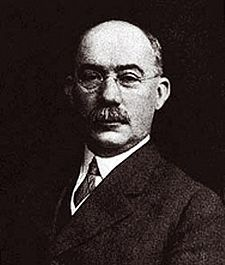
\includegraphics[width=\textwidth]{./graphics/henry-gantt}
\caption{Henry Laurence Gantt, A.B., M.E. (1861 - 23 November 1919) was an American mechanical engineer and management consultant who is most famous for developing the Gantt chart in the 1910s.
These Gantt charts were employed on major infrastructure projects including the Hoover Dam and Interstate highway system and continue to be an important tool in project management.}
\end{marginfigure}


These charts who are produced using Primavera by the Planning Department is
virtually our only tool that communicates the MEP sequence of works to the
rest of the Construction Team. None of the other methods that we have 
discussed handles this intercommunication. During construction though
experienced Construction Managers would normally revert to simpler tabular
or visual methods.

A simple gantt chart (more of a bar chart) can be used to define longer period
activities, that can establish targets. This does not show interdependencies
of activities and for which a more complicated version should be prepared by
the Project Planner. It is important also to bear in mind that if the works 
are delayed for reasons other than owr own (i.e., for example by late information
or by changes) unless there is a good document illustrating these delays it is
extremely difficult to justify the delays.


\begin{fullwidth}
\begin{figure*}[htbp]
\newcommand{\gbar}[3]{\ganttbar[crosshatch, color=orange]{#1}{#2}{#3}}

\definecolor{lightgray}{rgb}{0.7,0.7,0.7}
%% #1 11 rows deep
%% #2 24 cells wide

%% Define short-cuts for months
%%


\def\gantscale#1{}

\newcounter{acount}
\setcounter{acount}{0}
\stepcounter{acount}
\addtocounter{acount}{10}



%\ifnum\theacount>10 number is greater than ten \else number is less than ten\fi


%% Define the months just in case they have not been set
%% before. This needs to be internationalized.
\def\mon#1{\ifcase#1\or%
  Jan\or Feb\or Mar\or Apr\or May\or Jun\or%
  Jul\or Aug\or Sept\or Oct\or Nov\or Dec\else Error 
\fi}


%% a helper macro to add a comma and a space to make the
%% code later on a bit more cleaner

\def\addcomma{, }

%% We define a new counter for looping through the months
%% in order to create the calendar on top
%% this will need to be expanded later 
%\newcounter{monthcount}
%\setcounter{monthcount}{1}
%\whiledo{\value{monthcount}<12}
%  {%
%   \mon{\themonthcount}%
   % adds comma except last one
 %  \ifnum\themonthcount<11 \addcomma\else\relax\fi %
   
  % \stepcounter{monthcount}% 
  %}


%% prints date
%\mon{\numexpr 1+3\relax} \intcalcAdd{\number\year}{1} \relax

%% Global setup
%% 

\xdef\monthstoplot{40}
\xdef\linesdeep{9}

%% Chart drawn in the margins
%% This is the main routine for the chart

%% We define a scale
%
\def\ganttscale#1{#1}



\begin{gantt}[xunitlength=\ganttscale{0.25cm},  fontsize=\footnotesize, drawledgerline=false]{\linesdeep}{\monthstoplot}

%% Define the title of the chart
%%
%% 
\newcommand\GanttTitle[1]{
\ganttitle
    \titleelement{\textsc{#1}}{\monthstoplot}
\endganttitle
}


\GanttTitle{ECU and Black Steel Installation - All Towers}

\begin{ganttitle}
%% We define a new counter for looping through the months
%% in order to create the calendar on top
%% this will need to be expanded later 
\newcounter{monthcount}
\setcounter{monthcount}{1}
\whiledo{\value{monthcount}<11}
  {%
   \mon{\themonthcount}%
   % adds comma except last one
   %\ifnum\themonthcount<11 \addcomma\else\relax\fi %
   \titleelement{\mon{\themonthcount}}{4}
   \stepcounter{monthcount}% 
  }
 
\end{ganttitle}

%% We now loop to typeset the week labels
%% this needs to become more sophisticated
%% as some months do not have 4 weeks
\begin{ganttitle}
   \newcounter{weekcount}
   \setcounter{weekcount}{1}
   \whiledo{\value{weekcount}<11}
  {%
   \mon{\theweekcount}%
   \numtitle{1}{1}{4}{1}
   \stepcounter{weekcount}% 
  }      
\end{ganttitle}
 
%% We define some new colors
\definecolor{red}{rgb}{1,0,0}
% activities are plotted here
\xdef\prop{crosshatch, color=orange}

\ganttbar[\prop]{Rotana }{0}{14}
\ganttbar[crosshatch, color=gray]{Rotana - commissioning}{15}{6}


\ganttbar[crosshatch, color=DarkGreen]{Shangrila}{4}{14}
\ganttbar[crosshatch, color=gray]{Shangrila - commissioning}{19}{6}



\ganttbar[crosshatch, color=DarkGreen]{Merweb}{18}{6}
\ganttbar[crosshatch, color=Gray]{Merweb - commissioning}{24}{3}

\end{gantt}

\caption{All three Towers ECU and black steel installation and commissioning program. Planning provides a safety factor for all Towers for more than two months. We have also allowed for a longer than normal commissioning period in case we are faced with unforseen problems during commissioning.}
\label{plan}
\end{figure*}

\end{fullwidth}



%   
%\section{The gantt package}
%
%In the following you will find a short description of environments and commands: 
%
%The gantt environment draws the canvas of a gantt figure (realized as tikzpicture)
%The usage is |begin{gantt}[...]{no of Tasks to plot}{no of time slots}|
%The optional argument |[...]| can be filled in a |key=value| syntax, using one or more of the following keys:
%
%\begin{description}
%\item [xunitlength]  length of one time slot (default: 1 cm)
%\item [fontsize] fontsize of labels (default: |\normalsize|)
%\item [titlefontsize] fontsize of title section (default: |\small|)
%\item [drawledgerline] Switch to enable/disable the drawing of horizontal ledger lines (default value: false)
%\item [ganttitle] is the environment for drawing the title section
%\item [titleelement] draws one element of the title
%usage: |\titleelement{label}{length}}|
%\end{description}
%
%
%
%
%The \cmd{numtitle} draws a numbered sequence of title elements:
%usage: 
%
%\begin{teX}
%\numtitle{start number}{increment}{end number}{length of each title element}
%\end{teX}
%
%\cmd{ganttbar} draws a single, unconnected bar for representing a task
%usage: 
%
%\begin{teX}
%\ganttbar[pattern]{label}{start}{length}
%\end{teX}
%
%where the optional pattern argument is a tikz pattern, nice patterns for tasks are: 
%north west lines (default), north east lines, crosshatch, crosshatch dots, grid, ...
%
%
%\begin{verbatim}
%\cmd{ganttcon} draws an arrow between to bars with specified coordinates
%usage: \ganttbar{startx}{starty}{endx}{endy}
%
%\ganttbarcon draws a single bar \textit{and} connects the bar with the previous bar for consecutive tasks
%usage: 
%
%\begin{teX}
%\ganttbar[pattern]{label}{start}{length}
%\end{teX}
%
%where the optional pattern argument is a tikz pattern, nice patterns for tasks are: north west lines (default), north east lines, crosshatch, crosshatch dots, grid.
%
%\ganttgroup draws a bar to group tasks
%usage: \ganttgroup{label}{start}{length}
%
%\end{verbatim}
%\section{Physical completion}

%\label{g:test}
%
%\numberLineAt{10}
%\begin{teX}
%\def\mon#1{\ifcase#1\or%
%  Jan\or Feb\or Mar\or Apr\or May\or Jun\or%
%  Jul\or Aug\or Sept\or Oct\or Nov\or Dec\else Error 
%\fi}
%\end{teX}











%These are notes for the gantt chart


\section*{Responsibilities}

Planning spans across all lines of management. Table indicates the type of plans
required and who is responsible to produce them.

\begin{tabular}{lllll}
\toprule
item  &Description            &Prepare   &Check &Approve \\
\midrule
1 &Project Plan               &Planner   &PMs   &Pro. Director\\
2 &6-week look aheads         &Section eng. &PM  &--\\ 
3 &Graphical monitoring plans &Section Eng. &PM  &--\\
4 &Drawings Planning          &CAD Manager  &DM  &PD\\
5 &Materials Planning         &MCD Manager  &PM  &PD\\
6 &Mobilization/demobilization &Planner     &HR  &PD\\
7 &Documentation Plan         &Planner      &DM  &PD\\
8 &Claims                     &Comm.Manager &    &PD\\
\bottomrule
\end{tabular}


\section*{Delays}

Delays and changes to planning are inevitable. As you will recall one of the main 
purpose for developing plans in the first place is to be able to estimate and predict
the impact of events on the end date of the Project. It is the responsibility of the 
Engineer in charge and the Project Manager to identify these delays and appropriate
action be taken to mitigate them, either by requesting more resources to accelerate
the works - once the constraints are removed - or by requesting for an extension
of time.

























